\chapter{Bases technologiques}
Ce chapitre permet de présenter quelques bases théoriques nécessaires à la bonne compréhension de ce travail. 

\section{Traitement d'images}
\subsection{Représentation d'une image}\label{techno.traitement.repr}
Une image est formée de pixel. La figure \ref{fig:pixels} présente une image d'une taille de 104x71 pixels, où ceux-ci peuvent donc être distingués les uns des autres.

\begin{figure}[ht]
    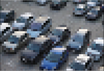
\includegraphics[width=50mm]{img/bases_technologiques/pixels.png}
    \centering
    \caption{Image de faible définition dont les pixels sont apparents}
    \label{fig:pixels} 
\end{figure}

Chaque pixel d'une image couleur est généralement constitué de 3 valeurs\footnote{Parfois, une composante de transparence peut aussi être présente. Dans certains cas bien spécifiques, il peut même être possible d'y inclure des composantes telles que la profondeur (la distance entre la caméra et l'objet désigné par le pixel), ou encore la température (caméra thermique).}: une composante rouge, une verte et une bleue, qui permet de décrire la couleur associé à ce pixel. En traitement d'image, ces composantes RGB\footnote{\textit{RGB}: \textit{Red Green Blue} pour \textit{rouge vert bleu}} sont souvent décrites comme des canaux\footnote{\textit{channel}, mot anglais, est aussi utilisé.} différents.

\begin{figure}[ht]
    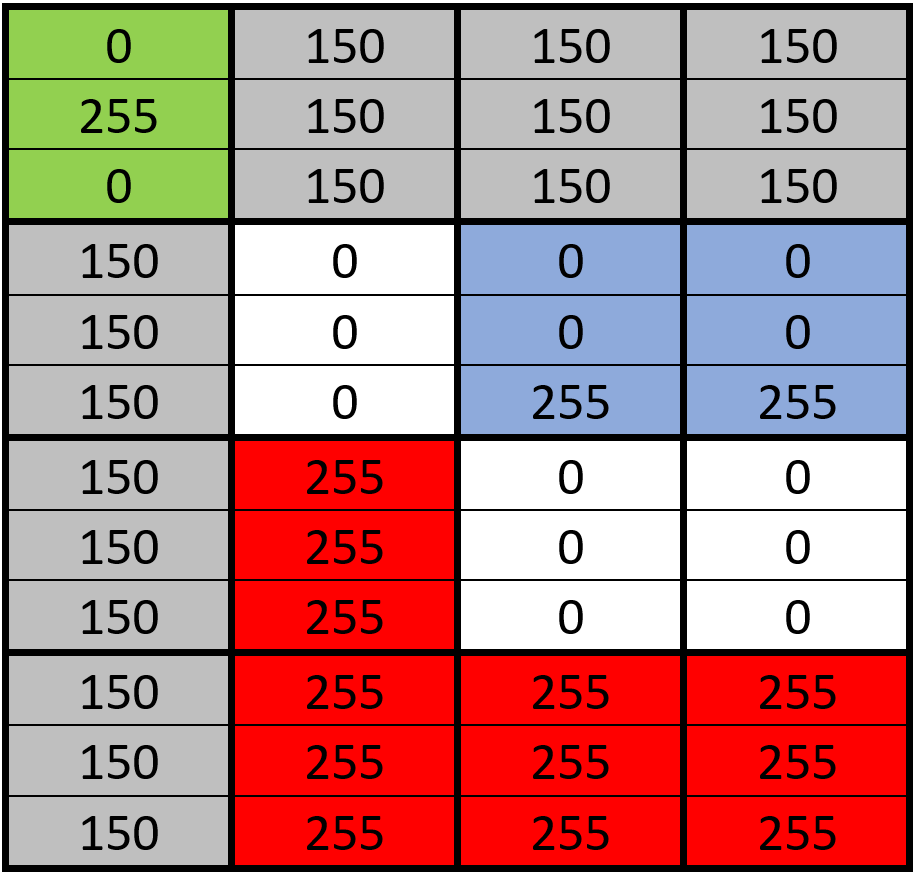
\includegraphics[width=50mm]{img/bases_technologiques/images_pixels.png}
    \centering
    \caption{Représentation d'une image couleur 4x4 pixels et les composantes rouges, vertes, et bleues}
\end{figure}

Une image couleur peut donc être représentée en mémoire à l'aide d'un tableau à 3 dimensions. 2 normes différentes peuvent être utilisées:
\begin{description}
    \item[Canal en premier (\textit{channel first})] Le canal est désigné par la première dimension. Ainsi, pour une image couleur de 4x4 pixels, le tableau est de la forme 3x4x4.
    \item[Canal en dernier (\textit{channel last})] Le canal est désigné par la dernière dimension. Pour une image couleur de 4x4 pixel, le tableau est de la forme 4x4x3.
\end{description}

Dans ce projet, il a été défini que le format \textit{canal en dernier} sera utilisé en priorité. 

\subsubsection{Espace de couleur}\label{techno.traitement.repr.coul}
En section précédente, le format RGB a été présenté. Il est cependant important de noter qu'il existe d'autres modèles permettant de représenter une couleur. Notamment, le modèle HSV (\textit{Hue, Saturation, Value}, en français \textit{TSV} pour \textit{teinte, saturation, valeur}) a été utilisé dans ce travail. \autocite{wiki:HSV} 

\begin{figure}[ht]
    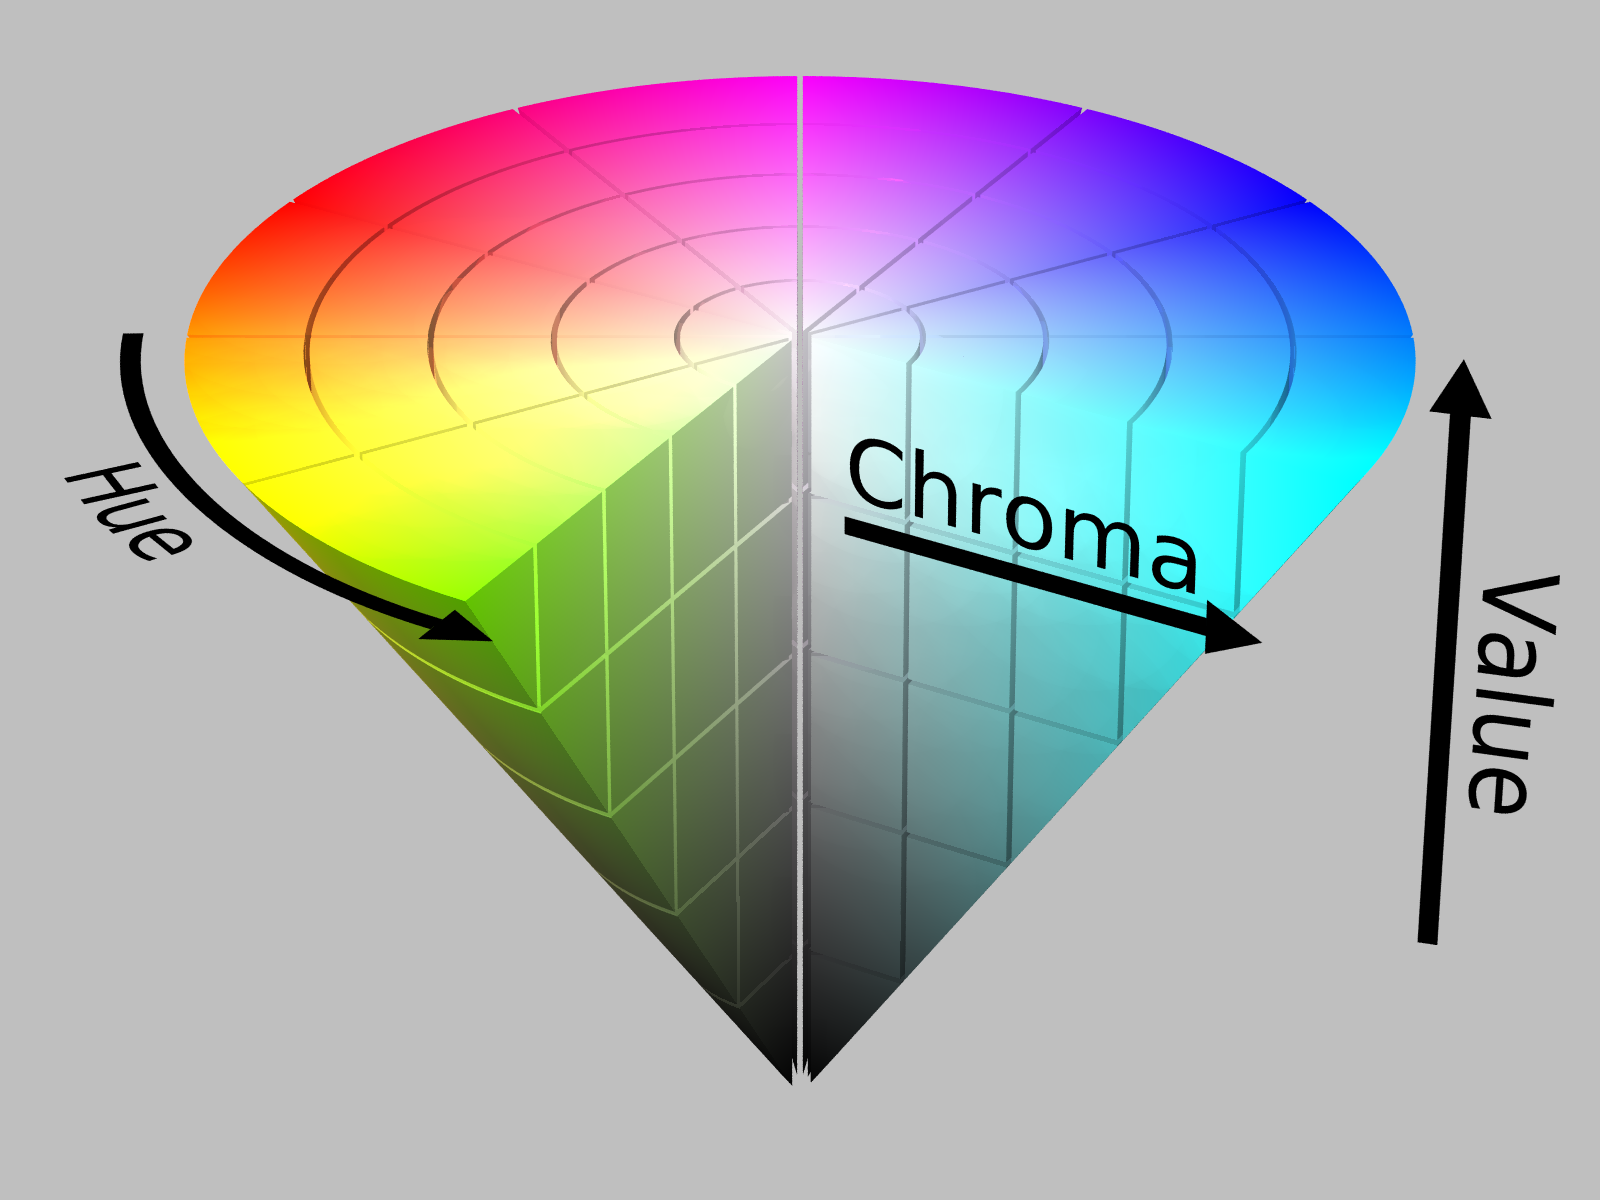
\includegraphics[width=70mm]{img/bases_technologiques/HSV.png}
    \centering
    \captionsource{Cône représentant l'espace HSV. Ici, la saturation est désignée par le terme \textit{Chroma}}{wiki:HSV}
\end{figure}

La teinte d'une couleur pouvant être obtenue grâce à l'aide d'un canal unique, cette représentation peut sembler idéale dans certains cas, permettant de mieux distinguer les couleurs entre elles. Notamment, cet espace de couleur a été utilisé lors des tests de détection de bords tel que décrit en section \ref{conception.traitement} \itnameref{conception.traitement}.

\subsection{Sous-échantillonnage}
Une image d'un certain nombre de pixel en largeur et en hauteur peut être redimensionnée. En traitement d'images\footnote{Le sur- et sous-échantillonnage sont en réalité utilisés pour toutes données décrites à l'aide d'échantillons ou une discrétisation, comme par exemple les fichiers audios.}, on parle de:
\begin{description}
    \item[Sur-échantillonnage (\textit{Oversampling})] La résolution de l'image est augmentée, le nombre de pixels qui y sont présents est donc supérieur. 
    \item[Sous-échantillonnage (\textit{Downsampling})] La résolution de l'image est réduite, le nombre de pixels qui y sont présents est donc diminué. 
\end{description}

Il est important de noter que la réduction de la résolution d'une image induit irrémédiablement à une perte d'information. 


\subsection{Détection de bord}\label{techno.traitement.bord}
Certains filtres permettent de mettre en valeur sur une images les bords des objets. Il sont souvent basés sur des matrices de convolutions. Celles-ci sont décrites plus amplement en section en section \ref{techno.traitement.convolution} \itnameref{techno.traitement.convolution}. 

\begin{figure}[ht]
    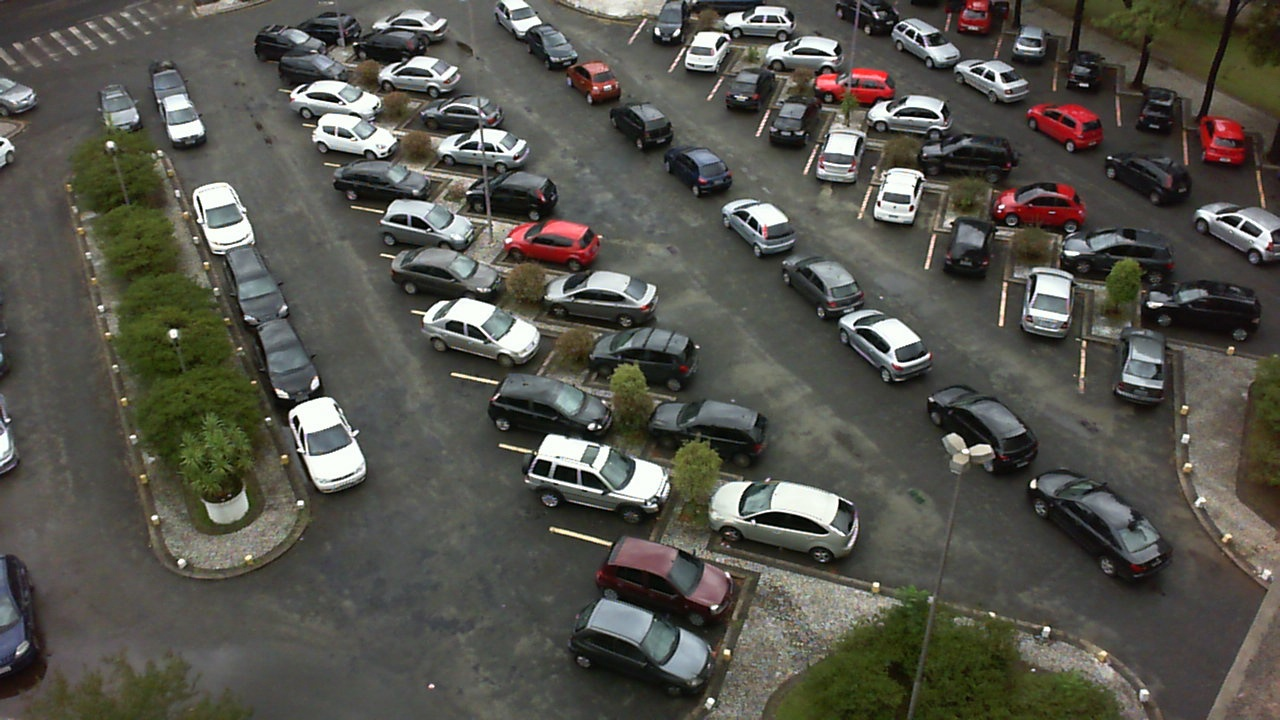
\includegraphics[width=80mm]{img/conception/pklot_park.jpg}
    \centering
    \captionsource{Image de parking avant détection de bord}{data:pklot}
\end{figure}

\begin{figure}[ht]
    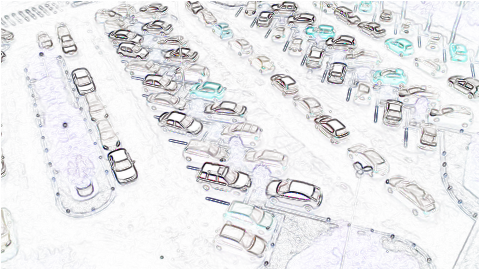
\includegraphics[width=80mm]{img/conception/image_process/downsample-edge/4.png}
    \centering
    \captionsource{Image de parking après détection de bord}{data:pklot}
\end{figure}

Ces filtres sont généralement appliqués sur des images noires et blanches. Cependant, il est possible de séparer une image couleur par canal, et d'appliquer le filtre sur chacun de ceux-ci. C'est ce qui a été fait dans ce projet.


\section{Réseau de neurones à convolutions}
\subsection{Apprentissage automatique (\textit{Machine Learning})}
Le \textit{Machine Learning} est un sous-domaine de l'intelligence artificielle. Comme son nom l'indique, il permet à une machine d'apprendre par divers moyens statistiques et automatiques.\autocite{wiki:ML} Ainsi, un algorithme permettant de réaliser une certaine tâche n'est pas directement défini par le développeur, mais "déduit" par apprentissage automatique.

Dans le cadre de ce TB, ce sont des algorithmes de type supervisé qui sont utilisés. L'apprentissage est effectué à l'aide de données labélisées. On distingue donc:
\begin{description}
    \item[Les données] Dans ce projet, il s'agit avant tout des images de parking. 
    \item[Les labels] Il s'agit de la sortie de l'algorithme qui est souhaité en fonction des données en entrée. Dans l'absolu ici, il s'agit de connaître le taux d'occupation du parking pour une image de parking donnée.
\end{description}

\subsection{Réseau de neurones}
Dans ce projet, les algorithmes utilisés se basent sur des réseaux de neurones. Cette section permet d'en présenter le fonctionnement général et l'application de ceux-ci dans le cadre de ce TB.
\begin{figure}[ht]
    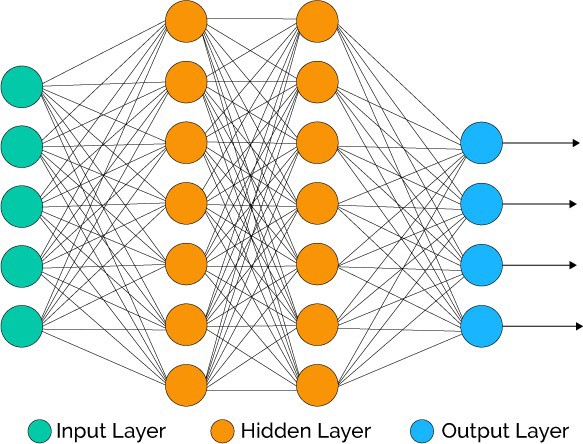
\includegraphics[width=80mm]{img/bases_technologiques/NN.jpg}
    \centering
    \captionsource{Exemple de réseau de neurones}{info:NN}
    \label{fig:nn}
\end{figure}

La figure \ref{fig:nn} présente une représentation minimale d'un réseau de neurone. On distinguera 3 couches, où chacune contient un certain nombre de neurones:
\begin{description}
    \item[Couche d'entrée (\textit{Input layer})] Chaque neurone de cette couche représente une partie des données d'entrées. Il est possible de faire un certain parallèle avec ce projet, où la couche d'entrée représente une image, et chaque neurone les pixels de celle-ci. Il faut cependant noter qu'avec un réseau de neurones à convolution (ce qui est utilisé dans ce projet), les choses sont légèrement différentes comme il sera possible de le voir en section \ref{techno.nn.convolution}.
    \item[Couche de sortie (\textit{Output layer})] Chaque neurone de cette couche représente une sortie de l'algorithme qu'on souhaite obtenir. Bien que dans l'absolu, il est souhaité de connaître le nombre de voitures présentes dans un parking (un seul neurone de sortie serait suffisant), il sera vu en section \ref{techno.nn.object} qu'il y en aura généralement plusieurs.
    \item[Couches cachées (\textit{Hidden layers})] Elles permettent de mettre en relation les données d'entrées et les sorties voulues, ce dans le but, après entrainement, de "déduire" certaines caractéristiques des données d'entrées.
\end{description}

L'étape d'entrainement consiste à utiliser les données labélisées sur un réseau de neurones. Dans le cadre de ce projet, une image de parking est mise en entrée du réseau, ainsi qu'indirectement le nombre de voitures présentes dans l'image en sortie. Les paramètres du modèles sont modifiés itérativement, au fil des images présentent dans le \textit{dataset}.

\subsection{Réseau de neurones à convolutions}\label{techno.nn.convolution}
A un réseau de neurones conventionnel, il est possible d'y ajouter des couches de convolutions. 

\begin{figure}[ht]
    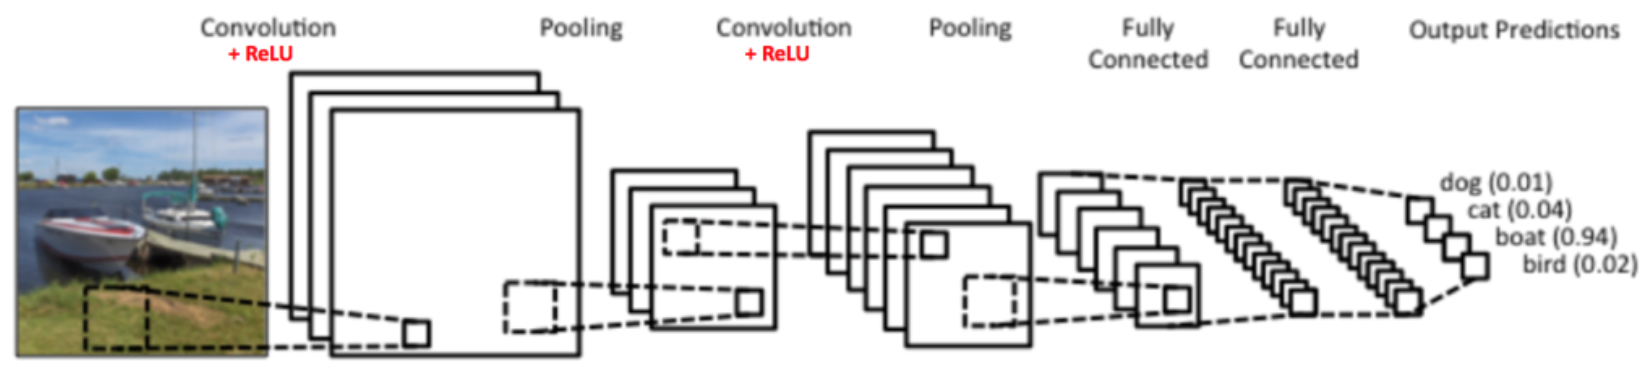
\includegraphics[width=120mm]{img/bases_technologiques/cnn.png}
    \centering
    \captionsource{Exemple de réseau de neurones à convolutions}{info:convnet}
    \label{fig:cnn}
\end{figure}

Une couche de convolution consiste en un certain nombre de filtres, qui seront appliqués à une image. D'une image entrante dans cette couche, on y applique une convolution. En sortie, une nouvelle image, filtrée, est générée.

Pour résumer, une matrice de convolution décrit un filtre. Cette matrice est appliquée sur l'ensemble des pixels d'une image. Une fois ce filtre appliqué, chacun des pixels de cette image en est donc modifié. Une couche de convolutions transforme donc des images d'entrées en image de sorties filtrées.

Il semblait nécessaire et important de décrire rapidement le fonctionnement de ces matrices de convolutions afin de faire le parallèle avec la détection de bords qui a été décrites en section \ref{techno.traitement.bord} \itnameref{techno.traitement.bord}. En effet, la détection de bord consiste en une matrice de convolution définie qui sera appliquée sur une image. En \textit{Machine Learning}, les matrices de convolutions sont "déduites" au fur et à mesure des itérations. Ainsi, il est possible qu'un réseau de neurones à convolutions apprenne de lui-même à effectuer une détection de bord, si tel est nécessaire. C'est pourquoi, ce traitement peut accélérer l'apprentissage, mais ne semble pas dans l'absolu nécessaire.

\subsection{Détection d'objet}\label{techno.nn.object}

Une approche possible afin de résoudre le problème présenté est de chercher à détecter les voitures présentes dans l'image. Une fois ces objets détectés, il est suffisant ensuite de compter le nombre de voitures prédites par l'algorithme. 

Il faut noter qu'en général, ces algorithmes permettent de détecter plusieurs classes d'objets. Ainsi, ils peuvent parfois sembler excessivement complexes pour la tâche qui doit être effectuée dans le cadre de ce travail. Cependant, ces algorithmes sont ceux qui semblent fonctionner le mieux.

En général, ces algorithmes se basent sur des réseaux de neurones à convolutions tels que vu en section précédente. La première couche prend en entrée une image. La couche de sortie, quant à elle, dépends des architectures choisies. Il en existe beaucoup: ainsi, dans ce projet, le temps n'a permit de n'en tester que deux, et c'est ceux-ci qui sont présentés. Cependant, il est possible de noter que les architectures utilisées dans la détection d'objets sont souvent basées sur certains mêmes principes, où la présentation des deux méthodes suivantes permet de les résumer. 

\paragraph{Faster R-CNN}

L'architecture \textit{Faster R-CNN}\autocite{faster-rcnn} présentée en figure \ref{fig:faster-rcnn} consiste en 2 étapes. Dans un premier temps, un réseau de neurones à convolutions permet de rechercher les zones d'intérêts (\textit{Regions of Interest}). Par la suite, chacune de ces zones est évaluée par un second réseau de neurones, afin de définir si la région appartient à certaine classe, ou à aucune d'entre elles.

\begin{figure}[ht]
    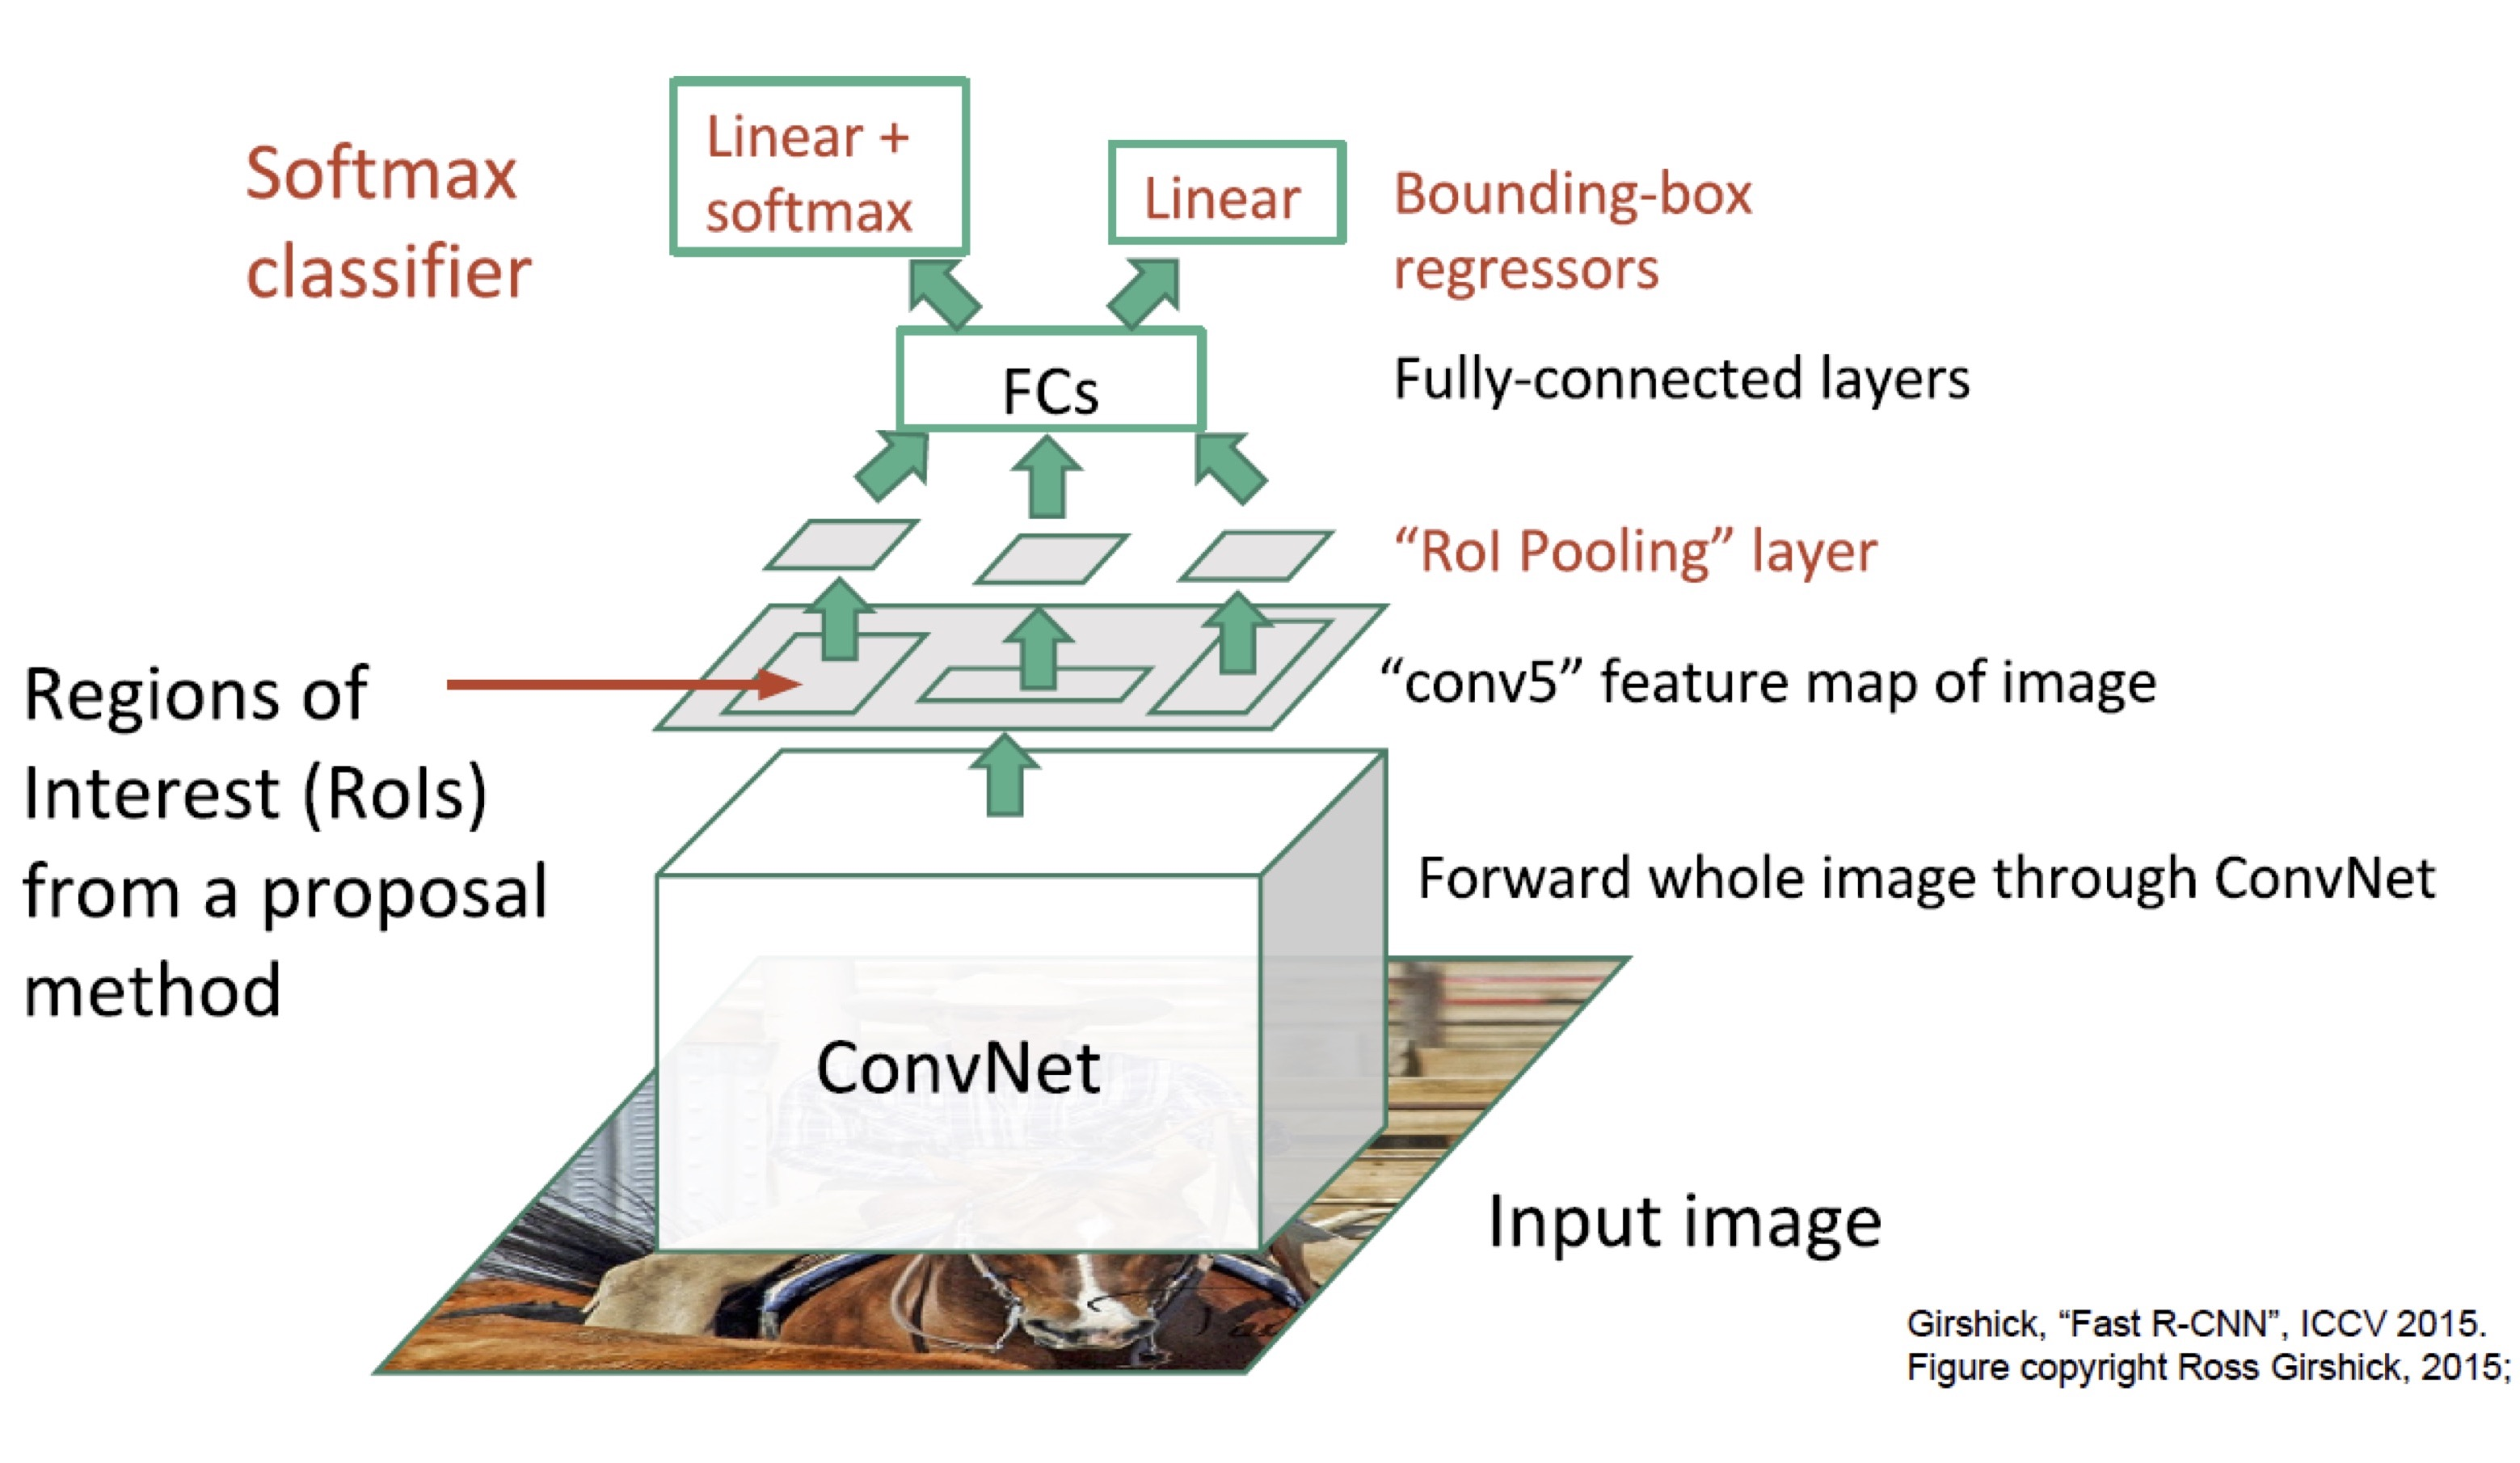
\includegraphics[width=120mm]{img/bases_technologiques/faster-rcnn.jpg}
    \centering
    \captionsource{Architecture \textit{Faster R-CNN}}{faster-rcnn}
    \label{fig:faster-rcnn}
\end{figure}


\paragraph{\textit{Yolo}}

L'architecture présentée par \textit{Yolo}\footnote{Yolo (You Only Look Once). \autocite{yolov3}} consiste en un unique réseau de neurones à convolutions. Conceptuellement, par couche de convolutions successive, l'image est finalement réduite à une grille la subdivisant. Chaque cellule de cette grille indique s'il y a un objet détecté dans l'image original à la position correspondante. 

\begin{figure}[ht]
    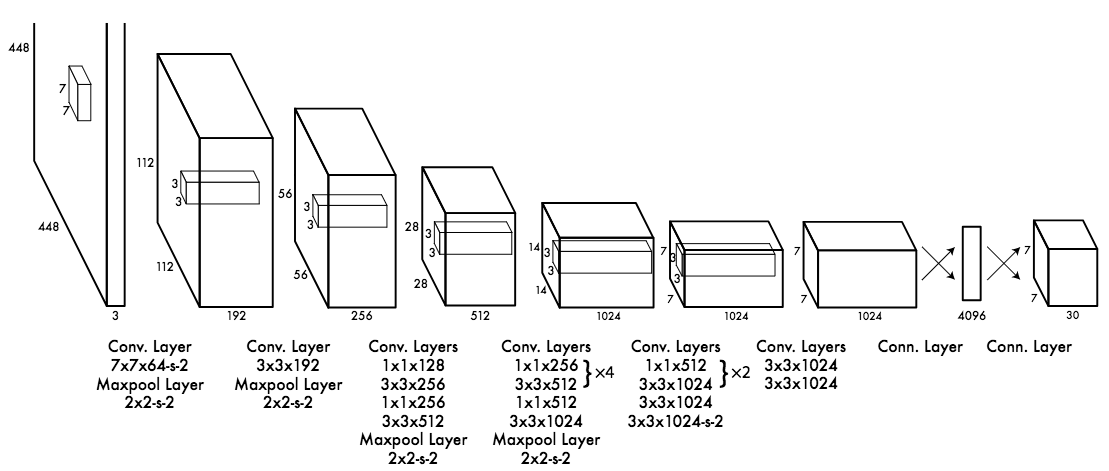
\includegraphics[width=120mm]{img/bases_technologiques/yolo.png}
    \centering
    \captionsource{Architecture \textit{Yolo}}{yolov3}
    \label{fig:yolo}
\end{figure}






\todo{Fenêtre glissante}